% Chapter 3, Topic _Linear Algebra_ Jim Hefferon
%  http://joshua.smcvt.edu/linearalgebra
%  2001-Jun-12
\topic{Markov Chains}
\index{Markov chain|(}

Here is a simple game:
a player bets on coin tosses, a dollar each time, 
and the game ends either when the player has no money 
or is up to five dollars. 
If the player starts with three dollars, what is the chance that the game 
takes at least five flips?
Twenty-five flips?

At any point, this player has either \$0, or \$1, \ldots, or \$5. 
We say that the player is in the 
\definend{state}\index{state} 
$s_0$, $s_1$, \ldots, or $s_5$.
In the game the player moves from state to state.
For instance,
a player now in state $s_3$ has on the next flip a $0.5$ chance of moving
to state $s_2$ and a $0.5$ chance of moving to $s_4$.
The boundary states are different; 
a player never leaves state~$s_0$ or state~$s_5$.

Let $p_{i}(n)$ be the probability that the player is in state $s_{i}$
after $n$ flips.
Then for instance the probability of being in state~$s_0$ 
after flip~$n+1$ is
$p_{0}(n+1)=p_{0}(n)+0.5\cdot p_{1}(n)$.
This equation summarizes.
\begin{equation*}
  % breqn didn't like this:
  % \begin{dmat}{D{.}{.}{1}D{.}{.}{1}D{.}{.}{1}D{.}{.}{1}D{.}{.}{1}D{.}{.}{1}}
    \begin{mat}
      1.0  &0.5  &0.0  &0.0  &0.0   &0.0  \\ 
      0.0  &0.0  &0.5  &0.0  &0.0   &0.0  \\ 
      0.0  &0.5  &0.0  &0.5  &0.0   &0.0  \\ 
      0.0  &0.0  &0.5  &0.0  &0.5   &0.0  \\ 
      0.0  &0.0  &0.0  &0.5  &0.0   &0.0  \\ 
      0.0  &0.0  &0.0  &0.0  &0.5   &1.0 
   \end{mat}  
   % \end{dmat}
   \colvec{p_{0}(n) \\ 
        p_{1}(n) \\
        p_{2}(n) \\
        p_{3}(n) \\
        p_{4}(n) \\
        p_{5}(n)}
   =\colvec{p_{0}(n+1) \\ 
        p_{1}(n+1) \\
        p_{2}(n+1) \\
        p_{3}(n+1) \\
        p_{4}(n+1) \\
        p_{5}(n+1)}
\end{equation*}

\textit{Sage} will compute the evolution of this game. 
\begin{lstlisting}
sage: M = matrix(RDF, [[1.0, 0.5, 0.0, 0.0, 0.0, 0.0],
....:                  [0.5, 0.0, 0.5, 0.0, 0.0, 0.0],
....:                  [0.0, 0.5, 0.0, 0.5, 0.0, 0.0],
....:                  [0.0, 0.0, 0.5, 0.0, 0.5, 0.0],
....:                  [0.0, 0.0, 0.0, 0.5, 0.0, 0.5],
....:                  [0.0, 0.0, 0.0, 0.0, 0.5, 1.0]])
sage: M = M.transpose()
sage: v0 = vector(RDF, [0.0, 0.0, 0.0, 1.0, 0.0, 0.0])
sage: v1 = v0*M
sage: v1
(0.0, 0.0, 0.5, 0.0, 0.5, 0.0)
sage: v2 = v1*M
sage: v2
(0.0, 0.25, 0.0, 0.5, 0.0, 0.25)  
\end{lstlisting}
(Two notes: (1)~\textit{Sage} can use various number systems to 
make the matrix entries and here we have used Real Double Float, and 
(2)~\textit{Sage} likes to do matrix multiplication from the right, 
as $\vec{v}\hspace{.1em}M$ instead of our usual $M\vec{v}$, 
so we needed to take the matrix's transpose.)

These are components of the resulting vectors.
\begin{center}
  \begin{tabular}{@{}c|ccccc@{\hspace*{5em}}c@{}}
    $n=0$
    &\multicolumn{1}{c}{$n=1$}
    &\multicolumn{1}{c}{$n=2$}
    &\multicolumn{1}{c}{$n=3$}
    &\multicolumn{1}{c}{$n=4$}
    &\multicolumn{1}{c}{$\cdots$}
    &$n=24$ \\ 
    \hline  
    $\begin{array}{l}
             0 \\ 0    \\  0   \\  1    \\  0    \\  0
     \end{array}$
    % breqn again
    % &$\dcolvec[1]{
    %    0      \\  0    \\  0.5  \\  0    \\  0.5    \\  0
    %      }$
    % &$\dcolvec[2]{
    %   0      \\  .25  \\ 0    \\ .5    \\  0     \\  .25
    %      }$
    % &$\dcolvec[3]{
    %     .125   \\   0   \\ .375 \\ 0     \\ .25    \\  .25
    %       }$
    % &$\dcolvec[4]{
    %     .125   \\ .1875 \\ 0    \\ .3125 \\ 0      \\ .375
    %       }$
    % &$\cdots$
    % &$\dcolvec[5]{
    %     .39600 \\ .00276   \\ 0    \\ .00447 \\ 0  \\ .59676
    %       }$
    &$\begin{array}{l}
       0      \\  0    \\  0.5  \\  0    \\  0.5    \\  0
      \end{array}$
    &$\begin{array}{l}
      0      \\  0.25  \\ 0    \\ 0.5    \\  0     \\  0.25
      \end{array}$
    &$\begin{array}{l}
        0.125   \\   0   \\ 0.375 \\ 0     \\ 0.25    \\  0.25
       \end{array}$
    &$\begin{array}{l}
        0.125   \\ 0.187\,5 \\ 0    \\ 0.312\,5 \\ 0      \\ 0.375
       \end{array}$
    &  % $\cdots$
    &$\begin{array}{l}
        0.396\,00 \\ 0.002\,76   \\ 0    \\ 0.004\,47 \\ 0  \\ 0.596\,76
      \end{array}$
  \end{tabular}  
\end{center}
This game is not likely to go on 
for long since the player quickly moves to an ending state.
For instance, after the fourth flip there is already a $0.50$~probability that 
the game is over.
% (Because a player who enters either of the boundary states never leaves, they
% are said to be \definend{absorbtive}.)\index{state!absorbtive}

This is a \definend{Markov chain}.\index{Markov chain!definition} 
Each vector is a 
\definend{probability vector},\index{vector!probability}%
\index{probability vector} whose entries are nonnegative real numbers that
sum to $1$.  
The matrix is a 
\definend{transition matrix}\index{matrix!transition}%
\index{transition matrix} 
or \definend{stochastic matrix},\index{matrix!stochastic}%
\index{stochastic matrix}  
whose entries are nonnegative reals and whose columns sum to $1$.

A characteristic feature of 
a Markov chain model is that it is
\definend{historyless}\index{historyless process}%
\index{Markov chain!historyless} in that  
the next state depends only on the current state,  
not on any prior ones.
Thus, a player
who arrives at $s_2$ by starting in state $s_3$ and 
then going to state~$s_2$ has exactly the same chance of 
moving next to $s_3$ as does a player whose history was to
start in $s_3$ then go to~$s_4$ then to~$s_3$ and then to~$s_2$.

Here is a Markov chain from sociology.
A study (\cite{MacdonaldRidge}, p.~202) 
divided occupations in the United Kingdom into three levels:
executives and professionals, 
supervisors and skilled manual workers, 
and unskilled workers.
They asked about 
two thousand men, ``At what level are you,
and at what level was your father when you were fourteen years old?''
Here the Markov model assumption about history
may seem reasonable\Dash 
we may guess that
while a parent's occupation has a direct influence on the occupation of the 
child, the grandparent's occupation likely has no such direct influence.
This summarizes the study's conclusions.
\begin{equation*}
  % breqn again
  % \begin{dmat}{D{.}{.}{2}D{.}{.}{2}D{.}{.}{2}}
  \begin{mat}
    .60  &.29  &.16  \\
    .26  &.37  &.27  \\
    .14  &.34  &.57
  \end{mat}  
  % \end{dmat}
  \colvec{p_{U}(n) \\ p_{M}(n) \\ p_{L}(n)}
  =\colvec{p_{U}(n+1) \\ p_{M}(n+1) \\ p_{L}(n+1)}
\end{equation*} 
For instance, looking at the middle class for the next generation, 
a child of an upper class worker has a $0.26$~probability of becoming
middle class, 
a child of a middle class worker has a $0.37$~chance of being middle
class, and 
a child of a lower class worker has a $0.27$ probability of
becoming middle class.

\textit{Sage} will compute the successive stages of this system
(the current class distribution is $\vec{v}_0$).
\begin{lstlisting}
sage: M = matrix(RDF, [[0.60, 0.29, 0.16],
....:                  [0.26, 0.37, 0.27],
....:                  [0.14, 0.34, 0.57]])
sage: M = M.transpose()
sage: v0 = vector(RDF, [0.12, 0.32, 0.56])
sage: v0*M
(0.2544, 0.3008, 0.4448)
sage: v0*M^2
(0.31104, 0.297536, 0.391424)
sage: v0*M^3
(0.33553728, 0.2966432, 0.36781952)  
\end{lstlisting}
Here are the next five generations.
They show upward mobility, especially in the 
first generation.
In particular, lower class shrinks a good bit.
\begin{center}
  % breqn again
  \begin{tabular}{c|ccccc}
    $n=0$  &$n=1$  &$n=2$  &$n=3$  &$n=4$  &$n=5$  \\ \hline
    $\begin{array}{l}
               .12 \\ .32  \\ .56
      \end{array}$
    &$\begin{array}{l}
               .25 \\ .30  \\ .44
       \end{array}$
    &$\begin{array}{l}
               .31 \\ .30  \\ .39  
       \end{array}$
    &$\begin{array}{l}
               .34 \\ .30  \\ .37  
       \end{array}$
    &$\begin{array}{l}
               .35 \\ .30 \\ .36  
       \end{array}$
    &$\begin{array}{l}
               .35 \\ .30  \\ .35  
       \end{array}$
  \end{tabular}
\end{center}

One more example.
In professional American baseball there are two leagues, the
American League and the National League.
At the end of the annual season 
the team winning the American League
and the team winning the National League play the World Series.
% what are these? (we follow [Brunner] but see also [Woodside]).
The winner is the first team to take four games.
That means that a series is in one of twenty-four states: 
$0$-$0$ (no games won yet by either team), 
$1$-$0$ (one game won for the American League
team and no games for the National League team), etc.

Consider a series with a probability $p$ that 
the American League team wins each game. 
We have this.
\begin{equation*}
  \begin{pmatrix}
    0      &0      &0      &0   &\ldots  \\
    p      &0      &0      &0   &\ldots  \\
    1-p    &0      &0      &0   &\ldots  \\
    0      &p      &0      &0   &\ldots  \\
    0      &1-p    &p      &0   &\ldots  \\
    0      &0      &1-p    &0   &\ldots  \\
    \vdots &\vdots &\vdots &\vdots
  \end{pmatrix}
  \colvec{p_{\text{0-0}}(n) \\ p_{\text{1-0}}(n) \\ p_{\text{0-1}}(n) \\
           p_{\text{2-0}}(n) \\ p_{\text{1-1}}(n) \\ p_{\text{0-2}}(n) \\ 
  \vdots }
  =
  \colvec{p_{\text{0-0}}(n+1) \\ p_{\text{1-0}}(n+1) \\ p_{\text{0-1}}(n+1) \\
           p_{\text{2-0}}(n+1) \\ p_{\text{1-1}}(n+1) \\ p_{\text{0-2}}(n+1) \\ 
           \vdots }
\end{equation*}
An especially interesting special case is when the teams are 
evenly matched, $p=0.50$.
This table below lists the
resulting components of the $n=0$ through $n=7$ vectors.
% (The code to generate this table in the computer algebra system
% Octave follows the exercises.)

Note that evenly-matched teams are likely to have a long series\Dash there
is a probability of $0.625$ that the series goes at least six games.

\begin{center}\small
\newcommand{\markovspacer}{\hspace{.8em}}
\begin{tabular}{@{}r|c@{\markovspacer}c@{\markovspacer}c@{\markovspacer}c@{\markovspacer}c@{\markovspacer}c@{\markovspacer}c@{\markovspacer}c@{}}
      &$n=0$  &$n=1$  &$n=2$  &$n=3$  &$n=4$  &$n=5$  &$n=6$  &$n=7$  \\ \hline
  $\begin{array}{@{}c@{}}
    0-0 \\
    1-0 \\
    0-1 \\
    2-0 \\
    1-1 \\
    0-2 \\
    3-0 \\
    2-1 \\
    1-2 \\
    0-3 \\
    4-0 \\
    3-1 \\
    2-2 \\
    1-3 \\
    0-4 \\
    4-1 \\
    3-2 \\
    2-3 \\
    1-4 \\
    4-2 \\
    3-3 \\
    2-4 \\
    4-3 \\
    3-4 
  \end{array}$
  &$\begin{array}{l}
     1 \\
     0 \\
     0 \\
     0 \\
     0 \\
     0 \\
     0 \\
     0 \\
     0 \\
     0 \\
     0 \\
     0 \\
     0 \\
     0 \\
     0 \\
     0 \\
     0 \\
     0 \\
     0 \\
     0 \\
     0 \\
     0 \\
     0 \\
     0 
   \end{array}$
  &$\begin{array}{l}
        0           \\
        0.5         \\
        0.5         \\
        0           \\
        0           \\
        0           \\
        0           \\
        0           \\
        0           \\
        0           \\
        0           \\
        0           \\
        0           \\
        0           \\
        0           \\
        0           \\
        0           \\
        0           \\
        0           \\
        0           \\
        0           \\
        0           \\
        0           \\
        0              
   \end{array}$
  &$\begin{array}{l}
        0           \\
        0           \\
        0           \\
        0.25        \\
        0.5         \\
        0.25        \\
        0           \\
        0           \\
        0           \\
        0           \\
        0           \\
        0           \\
        0           \\
        0           \\
        0           \\
        0           \\
        0           \\
        0           \\
        0           \\
        0           \\
        0           \\
        0           \\
        0           \\
        0              
   \end{array}$
  &$\begin{array}{l}
        0            \\
        0            \\
        0            \\
        0            \\
        0            \\
        0            \\
        0.125        \\
        0.375        \\
        0.375        \\
        0.125        \\
        0            \\
        0            \\
        0            \\
        0            \\
        0            \\
        0            \\
        0            \\
        0            \\
        0            \\
        0            \\
        0            \\
        0            \\
        0            \\
        0              
   \end{array}$
  &$\begin{array}{l}
        0              \\
        0              \\
        0              \\
        0              \\
        0              \\
        0              \\
        0              \\
        0              \\
        0              \\
        0              \\
        0.062\,5         \\
        0.25           \\
        0.375          \\
        0.25           \\
        0.062\,5         \\
        0              \\
        0              \\
        0              \\
        0              \\
        0              \\
        0              \\
        0              \\
        0              \\
        0                      
   \end{array}$
  &$\begin{array}{l}
        0              \\
        0              \\
        0              \\
        0              \\
        0              \\
        0              \\
        0              \\
        0              \\
        0              \\
        0              \\
        0.062\,5         \\
        0              \\
        0              \\
        0              \\
        0.062\,5         \\
        0.125          \\
        0.312\,5         \\
        0.312\,5         \\
        0.125          \\
        0              \\
        0              \\
        0              \\
        0              \\
        0                      
   \end{array}$
  &$\begin{array}{l}
        0               \\
        0               \\
        0               \\
        0               \\
        0               \\
        0               \\
        0               \\
        0               \\
        0               \\
        0               \\
        0.062\,5          \\
        0               \\
        0               \\
        0               \\
        0.062\,5          \\
        0.125           \\
        0               \\
        0               \\
        0.125           \\
        0.156\,25         \\
        0.312\,5          \\
        0.156\,25         \\
        0               \\
        0                      
   \end{array}$
  &$\begin{array}{l}
        0             \\
        0             \\
        0             \\
        0             \\
        0             \\
        0             \\
        0             \\
        0             \\
        0             \\
        0             \\
        0.062\,5        \\
        0             \\
        0             \\
        0             \\
        0.062\,5        \\
        0.125         \\
        0             \\
        0             \\
        0.125         \\
        0.156\,25       \\
        0             \\
        0.156\,25       \\
        0.156\,25       \\
        0.156\,25        
   \end{array}$
  % f-ing breqn
  % &$\begin{aligncolondecimal}{0}
  %    1 \\
  %    0 \\
  %    0 \\
  %    0 \\
  %    0 \\
  %    0 \\
  %    0 \\
  %    0 \\
  %    0 \\
  %    0 \\
  %    0 \\
  %    0 \\
  %    0 \\
  %    0 \\
  %    0 \\
  %    0 \\
  %    0 \\
  %    0 \\
  %    0 \\
  %    0 \\
  %    0 \\
  %    0 \\
  %    0 \\
  %    0 
  %  \end{aligncolondecimal}$
  % &$\begin{aligncolondecimal}{1}
  %       0           \\
  %       0.5         \\
  %       0.5         \\
  %       0           \\
  %       0           \\
  %       0           \\
  %       0           \\
  %       0           \\
  %       0           \\
  %       0           \\
  %       0           \\
  %       0           \\
  %       0           \\
  %       0           \\
  %       0           \\
  %       0           \\
  %       0           \\
  %       0           \\
  %       0           \\
  %       0           \\
  %       0           \\
  %       0           \\
  %       0           \\
  %       0              
  %  \end{aligncolondecimal}$
  % &$\begin{aligncolondecimal}{2}
  %       0           \\
  %       0           \\
  %       0           \\
  %       0.25        \\
  %       0.5         \\
  %       0.25        \\
  %       0           \\
  %       0           \\
  %       0           \\
  %       0           \\
  %       0           \\
  %       0           \\
  %       0           \\
  %       0           \\
  %       0           \\
  %       0           \\
  %       0           \\
  %       0           \\
  %       0           \\
  %       0           \\
  %       0           \\
  %       0           \\
  %       0           \\
  %       0              
  %  \end{aligncolondecimal}$
  % &$\begin{aligncolondecimal}{3}
  %       0            \\
  %       0            \\
  %       0            \\
  %       0            \\
  %       0            \\
  %       0            \\
  %       0.125        \\
  %       0.375        \\
  %       0.375        \\
  %       0.125        \\
  %       0            \\
  %       0            \\
  %       0            \\
  %       0            \\
  %       0            \\
  %       0            \\
  %       0            \\
  %       0            \\
  %       0            \\
  %       0            \\
  %       0            \\
  %       0            \\
  %       0            \\
  %       0              
  %  \end{aligncolondecimal}$
  % &$\begin{aligncolondecimal}{4}
  %       0              \\
  %       0              \\
  %       0              \\
  %       0              \\
  %       0              \\
  %       0              \\
  %       0              \\
  %       0              \\
  %       0              \\
  %       0              \\
  %       0.0625         \\
  %       0.25           \\
  %       0.375          \\
  %       0.25           \\
  %       0.0625         \\
  %       0              \\
  %       0              \\
  %       0              \\
  %       0              \\
  %       0              \\
  %       0              \\
  %       0              \\
  %       0              \\
  %       0                      
  %  \end{aligncolondecimal}$
  % &$\begin{aligncolondecimal}{4}
  %       0              \\
  %       0              \\
  %       0              \\
  %       0              \\
  %       0              \\
  %       0              \\
  %       0              \\
  %       0              \\
  %       0              \\
  %       0              \\
  %       0.0625         \\
  %       0              \\
  %       0              \\
  %       0              \\
  %       0.0625         \\
  %       0.125          \\
  %       0.3125         \\
  %       0.3125         \\
  %       0.125          \\
  %       0              \\
  %       0              \\
  %       0              \\
  %       0              \\
  %       0                      
  %  \end{aligncolondecimal}$
  % &$\begin{aligncolondecimal}{5}
  %       0               \\
  %       0               \\
  %       0               \\
  %       0               \\
  %       0               \\
  %       0               \\
  %       0               \\
  %       0               \\
  %       0               \\
  %       0               \\
  %       0.0625          \\
  %       0               \\
  %       0               \\
  %       0               \\
  %       0.0625          \\
  %       0.125           \\
  %       0               \\
  %       0               \\
  %       0.125           \\
  %       0.15625         \\
  %       0.3125          \\
  %       0.15625         \\
  %       0               \\
  %       0                      
  %  \end{aligncolondecimal}$
  % &$\begin{aligncolondecimal}{5}
  %       0             \\
  %       0             \\
  %       0             \\
  %       0             \\
  %       0             \\
  %       0             \\
  %       0             \\
  %       0             \\
  %       0             \\
  %       0             \\
  %       0.0625        \\
  %       0             \\
  %       0             \\
  %       0             \\
  %       0.0625        \\
  %       0.125         \\
  %       0             \\
  %       0             \\
  %       0.125         \\
  %       0.15625       \\
  %       0             \\
  %       0.15625       \\
  %       0.15625       \\
  %       0.15625        
  %  \end{aligncolondecimal}$
\end{tabular}
\end{center}

Markov chains are a 
widely used application of matrix operations.
They also  give us 
an example of the use of matrices where we do not consider
the significance of the maps represented by the matrices.
For more on Markov chains, there are many sources such as
\cite{KemenySnell} and \cite{Iosifescu}.

\begin{exercises}
  % \item[]\textit{Use a computer for these problems.
  %   You can, for instance, adapt the Octave script given below.}
  \item 
    These questions refer to the coin-flipping game.
    \begin{exparts}
     \partsitem Check the computations in the table at the end of the
       first paragraph.
     \partsitem Consider the second row of the vector table.
       Note that this row has alternating $0$'s.  
       Must $p_{1}(j)$ be $0$ when $j$ is odd?
       Prove that it must be, or produce a counterexample.
     \partsitem Perform a computational experiment to estimate
       the chance that the player ends at five dollars, 
       starting with one dollar, two dollars, and four dollars.
    \end{exparts}
    \begin{answer}
      \begin{exparts}
        \partsitem With this file \texttt{coin.m}
\begin{computercode}         
# Octave function for Markov coin game.  p is chance of going down.
function w = coin(p,v)
  q = 1-p;
  A=[1,p,0,0,0,0;
     0,0,p,0,0,0;
     0,q,0,p,0,0;
     0,0,q,0,p,0;
     0,0,0,q,0,0;
     0,0,0,0,q,1];
  w = A * v;
endfunction
\end{computercode}
         This Octave session produced the output given here. 
\begin{computercode}
octave:1> v0=[0;0;0;1;0;0]
v0 =
  0
  0
  0
  1
  0
  0
octave:2> p=.5
p = 0.50000
octave:3> v1=coin(p,v0)
v1 =
  0.00000
  0.00000
  0.50000
  0.00000
  0.50000
  0.00000
octave:4> v2=coin(p,v1)
v2 =
  0.00000
  0.25000
  0.00000
  0.50000
  0.00000
  0.25000
\end{computercode}
This continued for too many steps to list here.
\begin{computercode}
octave:26> v24=coin(p,v23)
v24 =
  0.39600
  0.00276
  0.00000
  0.00447
  0.00000
  0.59676
\end{computercode}        
        \partsitem Using these formulas
          \begin{alignat*}{2}
             p_{1}(n+1) &= 0.5\cdot p_{2}(n)
             &\qquad
             p_{2}(n+1) &= 0.5\cdot p_{1}(n)+0.5\cdot p_{3}(n)
                                                              \\
             p_{3}(n+1) &= 0.5\cdot p_{2}(n)+0.5\cdot p_{4}(n)
             &\qquad
             p_{5}(n+1) &= 0.5\cdot p_{4}(n)             
          \end{alignat*}
          and these initial conditions
          \begin{equation*}
            \colvec{p_{0}(0) \\ p_{1}(0) \\ p_{2}(0) \\ p_{3}(0) \\ 
                        p_{4}(0) \\ p_{5}(0)}
            =
            \colvec{0 \\ 0 \\ 0 \\ 1 \\ 
                        0 \\ 0}
          \end{equation*} 
          we will prove by induction that when $n$ is odd then 
          $p_{1}(n)=p_{3}(n)=0$ and when $n$ is even then
          $p_{2}(n)=p_{4}(n)=0$.
          Note first that this is true in the $n=0$ base case by the initial
          conditions.
          For the inductive step, suppose that it is true in the
          $n=0$, $n=1$, \ldots, $n=k$~cases and consider the $n=k+1$ case.
          If $k+1$ is odd then the two
          \begin{align*}
             p_{1}(k+1) &= 0.5\cdot p_{2}(k)=0.5\cdot 0=0
                                                          \\
             p_{3}(k+1) &=0.5\cdot p_{2}(k)+0.5\cdot p_{4}(k)
                        =0.5\cdot 0+0.5\cdot 0
                        =0
          \end{align*}
          follow from the inductive hypothesis that 
          $p_{2}(k)=p_{4}(k)=0$ since $k$ is even.
          The case where $k+1$ is even is similar.
        \partsitem We can use, say, $n=100$.
          This Octave session
\begin{computercode}
octave:1> B=[1,.5,0,0,0,0;
>             0,0,.5,0,0,0;
>             0,.5,0,.5,0,0;
>             0,0,.5,0,.5,0;
>             0,0,0,.5,0,0;
>             0,0,0,0,.5,1];
octave:2> B100=B**100
B100 =
  1.00000  0.80000  0.60000  0.40000  0.20000  0.00000
  0.00000  0.00000  0.00000  0.00000  0.00000  0.00000
  0.00000  0.00000  0.00000  0.00000  0.00000  0.00000
  0.00000  0.00000  0.00000  0.00000  0.00000  0.00000
  0.00000  0.00000  0.00000  0.00000  0.00000  0.00000
  0.00000  0.20000  0.40000  0.60000  0.80000  1.00000
octave:3> B100*[0;1;0;0;0;0]
octave:4> B100*[0;1;0;0;0;0]
octave:5> B100*[0;0;0;1;0;0]
octave:6> B100*[0;1;0;0;0;0]
\end{computercode}
        yields these outputs.
        \begin{equation*}
          \begin{array}{r|*{4}{c}}
            \multicolumn{1}{r}{\textit{starting with:}}
            &\text{\$1}  &\text{\$2}  &\text{\$3}  &\text{\$4} \\ 
             \hline
               \begin{array}{c}
                 s_{0}(100) \\
                 s_{1}(100) \\
                 s_{2}(100) \\
                 s_{3}(100) \\
                 s_{4}(100) \\
                 s_{5}(100)
               \end{array}
               &\begin{aligncolondecimal}{5}
                 0.80000 \\
                 0.00000 \\
                 0.00000 \\
                 0.00000 \\
                 0.00000 \\
                 0.20000
               \end{aligncolondecimal}
               &\begin{aligncolondecimal}{5}
                    0.60000 \\
                    0.00000 \\
                    0.00000 \\
                    0.00000 \\
                    0.00000 \\
                    0.40000         
               \end{aligncolondecimal}
               &\begin{aligncolondecimal}{5}
                      0.40000 \\
                      0.00000 \\
                      0.00000 \\
                      0.00000 \\
                      0.00000 \\
                      0.60000           
               \end{aligncolondecimal}
               &\begin{aligncolondecimal}{5}
                   0.20000 \\
                   0.00000 \\
                   0.00000 \\
                   0.00000 \\
                   0.00000 \\
                   0.80000        
               \end{aligncolondecimal}
          \end{array}
        \end{equation*}
      \end{exparts}
    \end{answer}
  \item 
    \cite{Feller} % , p.~424.
    We consider throws of a die, and say the system is in state $s_i$ if the
    largest number yet appearing on the die was $i$.
    \begin{exparts}
      \partsitem Give the transition matrix.
      \partsitem Start the system in state $s_1$, and run it
        for five throws.
        What is the vector at the end? 
    \end{exparts}
    \begin{answer}
      \begin{exparts}
        \partsitem From these equations
          \begin{equation*}
            \begin{linsys}{6}
              s_{1}(n)/6 &+ &0s_{2}(n) &+ &0s_{3}(n) 
                  &+ &0s_{4}(n) &+ &0s_{5}(n)  &+ &0s_{6}(n)  &= &s_{1}(n+1) \\
              s_{1}(n)/6 &+ &2s_{2}(n)/6 &+ &0s_{3}(n) 
                  &+ &0s_{4}(n) &+ &0s_{5}(n)  &+ &0s_{6}(n)  &= &s_{2}(n+1) \\
              s_{1}(n)/6 &+ &s_{2}(n)/6 &+ &3s_{3}(n)/6 
                  &+ &0s_{4}(n) &+ &0s_{5}(n)  &+ &0s_{6}(n)  &= &s_{3}(n+1) \\
              s_{1}(n)/6 &+ &s_{2}(n)/6 &+ &s_{3}(n)/6 
                  &+ &4s_{4}(n)/6 &+ &0s_{5}(n)  &+ &0s_{6}(n)  
                  &=  &s_{4}(n+1) \\
              s_{1}(n)/6 &+ &s_{2}(n)/6 &+ &s_{3}(n)/6 
                  &+ &s_{4}(n)/6 &+ &5s_{5}(n)/6  &+ &0s_{6}(n)  
                  &=  &s_{5}(n+1) \\
              s_{1}(n)/6 &+ &s_{2}(n)/6 &+ &s_{3}(n)/6 
                  &+ &s_{4}(n)/6 &+ &s_{5}(n)/6  &+ &6s_{6}(n)/6  
                  &=  &s_{6}(n+1) 
            \end{linsys}
          \end{equation*}
          We get this transition matrix.
          \begin{equation*}
            \begin{mat}
              1/6  &0   &0   &0   &0   &0  \\
              1/6  &2/6 &0   &0   &0   &0  \\
              1/6  &1/6 &3/6 &0   &0   &0  \\
              1/6  &1/6 &1/6 &4/6 &0   &0  \\
              1/6  &1/6 &1/6 &1/6 &5/6 &0  \\
              1/6  &1/6 &1/6 &1/6 &1/6 &6/6  
            \end{mat}
          \end{equation*}
       \partsitem This is the Octave session, 
         with outputs edited out and condensed into the table at the end.
\begin{computercode}
octave:1>   F=[1/6,  0,   0,   0,   0,   0;
>      1/6,  2/6, 0,   0,   0,   0; 
>      1/6,  1/6, 3/6, 0,   0,   0;  
>      1/6,  1/6, 1/6, 4/6, 0,   0; 
>      1/6,  1/6, 1/6, 1/6, 5/6, 0; 
>      1/6,  1/6, 1/6, 1/6, 1/6, 6/6];
octave:2> v0=[1;0;0;0;0;0]
octave:3> v1=F*v0
octave:4> v2=F*v1
octave:5> v3=F*v2
octave:6> v4=F*v3
octave:7> v5=F*v4
\end{computercode}
        These are the results.
        \begin{equation*}
          \begin{array}{c|*{5}{c}}
            \multicolumn{1}{c}{\ }
            &1  &2  &3  &4 &5  \\ 
            \hline
               \begin{aligncolondecimal}{0}
                   1 \\
                   0 \\
                   0 \\
                   0 \\
                   0 \\
                   0              
               \end{aligncolondecimal}
               &\begin{aligncolondecimal}{5}
                    0.16667 \\
                    0.16667 \\
                    0.16667 \\
                    0.16667 \\
                    0.16667 \\
                    0.16667         
               \end{aligncolondecimal}
               &\begin{aligncolondecimal}{6}
                   0.027778 \\
                   0.083333 \\
                   0.138889 \\
                   0.194444 \\
                   0.250000 \\
                   0.305556       
               \end{aligncolondecimal}
               &\begin{aligncolondecimal}{7}
                    0.0046296 \\
                    0.0324074 \\
                    0.0879630 \\
                    0.1712963 \\
                    0.2824074 \\
                    0.4212963       
               \end{aligncolondecimal}
               &\begin{aligncolondecimal}{8}
                    0.00077160 \\
                    0.01157407 \\
                    0.05015432 \\
                    0.13503086 \\
                    0.28472222 \\
                    0.51774691      
               \end{aligncolondecimal}
               &\begin{aligncolondecimal}{8}
                   0.00012860 \\
                   0.00398663 \\
                   0.02713477 \\
                   0.10043724 \\
                   0.27019033 \\
                   0.59812243     
               \end{aligncolondecimal}
          \end{array}
        \end{equation*}
      \end{exparts}
    \end{answer}
  \item 
    \cite{Kelton} % , p.~43
    There has been much interest in whether industries in the
    United States are moving from the Northeast and North Central regions to 
    the South and  West, motivated by the warmer climate, by lower wages, 
    and by less unionization.
    Here is the transition matrix for large firms in 
    Electric and Electronic Equipment.
    {\setlength\topsep{1pt plus 0.4pt minus 0.25pt}
    \begin{center}
      \begin{tabular}{c|ccccc}
            &\textit{NE}      
            &\textit{NC}      
            &\textit{S}      
            &\textit{W}      
            &\textit{Z}       \\ \hline
        \begin{tabular}{l}
           \textit{NE} \\
           \textit{NC} \\
           \textit{S}  \\
           \textit{W}  \\
           \textit{Z}  
        \end{tabular}
        &$\begin{array}{l}
           0.787  \\
           0      \\
           0      \\
           0      \\
           0.021
         \end{array}$
        &$\begin{array}{l}
           0      \\
           0.966  \\
           0.063  \\
           0      \\
           0.009
         \end{array}$
        &$\begin{array}{l}
           0      \\
           0.034  \\
           0.937  \\
           0.074  \\
           0.005
         \end{array}$
        &$\begin{array}{l}
           0.111  \\
           0      \\
           0      \\
           0.612  \\
           0.010
         \end{array}$
        &$\begin{array}{l}
           0.102  \\
           0      \\
           0      \\
           0.314  \\
           0.954    
         \end{array}$
        % breqn
        % &$\begin{aligncolondecimal}{3}
        %    0.787  \\
        %    0      \\
        %    0      \\
        %    0      \\
        %    0.021
        %  \end{aligncolondecimal}$
        % &$\begin{aligncolondecimal}{3}
        %    0      \\
        %    0.966  \\
        %    0.063  \\
        %    0      \\
        %    0.009
        %  \end{aligncolondecimal}$
        % &$\begin{aligncolondecimal}{3}
        %    0      \\
        %    0.034  \\
        %    0.937  \\
        %    0.074  \\
        %    0.005
        %  \end{aligncolondecimal}$
        % &$\begin{aligncolondecimal}{3}
        %    0.111  \\
        %    0      \\
        %    0      \\
        %    0.612  \\
        %    0.010
        %  \end{aligncolondecimal}$
        % &$\begin{aligncolondecimal}{3}
        %    0.102  \\
        %    0      \\
        %    0      \\
        %    0.314  \\
        %    0.954    
        %  \end{aligncolondecimal}$
      \end{tabular}
    \end{center}}
    For example, a firm in the Northeast region will be in the West region
    next year with probability $0.111$.
    (The \textit{Z} entry is a ``birth-death'' state.
     For instance, 
     with probability $0.102$ a large Electric and Electronic Equipment
     firm from the Northeast will move out of this system next year:~go
     out of business, move abroad, or move to another category of firm.
     There is a $0.021$ probability that a firm 
     in the \emph{National Census of Manufacturers}
     will move into Electronics, or be created, or move in from abroad, 
     into the Northeast.
     Finally, with probability $0.954$ a firm out of the categories
     will stay out, according to this research.)
    \begin{exparts}
      \partsitem Does the Markov model assumption of lack of history seem
        justified?
      \partsitem Assume that the initial distribution is even, except that
        the value at $Z$ is $0.9$.
        Compute the vectors for $n=1$ through $n=4$.
      \partsitem Suppose that the initial distribution is this.
        \begin{center}
          \begin{tabular}{ccccc}
              \textit{NE}      
              &\textit{NC}      
              &\textit{S}       
              &\textit{W}       
              &\textit{Z}       \\ \hline
              $0.0000$ &$0.6522$ &$0.3478$ &$0.0000$ &$0.0000$
          \end{tabular}
        \end{center}
        Calculate the distributions for $n=1$ through $n=4$.
      \partsitem Find the distribution for $n=50$ and $n=51$.
        Has the system settled down to an equilibrium?
    \end{exparts}
    \begin{answer}
     \begin{exparts}
      \partsitem It does seem reasonable that, while the firm's present 
        location should strongly influence where it is next time (for 
        instance, whether it stays), any locations in the prior stages should
        have little influence.
        That is, while a company may move or stay because of where it is, 
        it is unlikely to move or stay because of where it was.
      \partsitem This is  the Octave session, slightly edited, with the outputs
        put together in a table at the end.
\begin{lstlisting}
octave:1> M=[.787,0,0,.111,.102;
>            0,.966,.034,0,0;
>            0,.063,.937,0,0;
>            0,0,.074,.612,.314;
>            .021,.009,.005,.010,.954]
M =
  0.78700  0.00000  0.00000  0.11100  0.10200
  0.00000  0.96600  0.03400  0.00000  0.00000
  0.00000  0.06300  0.93700  0.00000  0.00000
  0.00000  0.00000  0.07400  0.61200  0.31400
  0.02100  0.00900  0.00500  0.01000  0.95400
octave:2> v0=[.025;.025;.025;.025;.900]
octave:3> v1=M*v0
octave:4> v2=M*v1
octave:5> v3=M*v2
octave:6> v4=M*v3
\end{lstlisting}
        This table summarizes.
        \begin{center}
           \begin{tabular}{c|cccc}
             $\vec{p}_0$   &$\vec{p}_1$    &$\vec{p}_2$   
                    &$\vec{p}_3$   &$\vec{p}_4$    \\ \hline
             $\left(\begin{aligncolondecimal}{6}
                    0.025000 \\ 
                    0.025000 \\ 
                    0.025000 \\ 
                    0.025000 \\ 
                    0.900000        
              \end{aligncolondecimal}\right)$
             &$\left(\begin{aligncolondecimal}{6}
                  0.114250 \\
                  0.025000 \\
                  0.025000 \\
                  0.299750 \\
                  0.859725      
              \end{aligncolondecimal}\right)$
             &$\left(\begin{aligncolondecimal}{6}
                  0.210879 \\
                  0.025000 \\
                  0.025000 \\
                  0.455251 \\
                  0.825924      
              \end{aligncolondecimal}\right)$
             &$\left(\begin{aligncolondecimal}{6}
                  0.300739 \\
                  0.025000 \\
                  0.025000 \\
                  0.539804 \\
                  0.797263      
              \end{aligncolondecimal}\right)$
             &$\left(\begin{aligncolondecimal}{6}
                  0.377920 \\
                  0.025000 \\
                  0.025000 \\
                  0.582550 \\
                  0.772652      
              \end{aligncolondecimal}\right)$
           \end{tabular}
       \end{center} 
       \partsitem This is a continuation of the Octave session from
         the prior item.
\begin{lstlisting}
octave:7> p0=[.0000;.6522;.3478;.0000;.0000]
octave:8> p1=M*p0
octave:9> p2=M*p1
octave:10> p3=M*p2
octave:11> p4=M*p3
\end{lstlisting}
        This summarizes the output.
        \begin{center}
           \begin{tabular}{c|cccc}
             $\vec{p}_0$   &$\vec{p}_1$    &$\vec{p}_2$   
                    &$\vec{p}_3$   &$\vec{p}_4$    \\ \hline
             $\left(\begin{aligncolondecimal}{5}
                  0.00000 \\
                  0.65220 \\
                  0.34780 \\
                  0.00000 \\
                  0.00000       
              \end{aligncolondecimal}\right)$
             &$\left(\begin{aligncolondecimal}{5}
                  0.00000 \\
                  0.64185 \\
                  0.36698 \\
                  0.02574 \\
                  0.00761       
              \end{aligncolondecimal}\right)$
             &$\left(\begin{aligncolondecimal}{7}
                  0.0036329 \\
                  0.6325047 \\
                  0.3842942 \\
                  0.0452966 \\
                  0.0151277     
              \end{aligncolondecimal}\right)$
             &$\left(\begin{aligncolondecimal}{7}
                  0.0094301 \\
                  0.6240656 \\
                  0.3999315 \\
                  0.0609094 \\
                  0.0225751     
              \end{aligncolondecimal}\right)$
             &$\left(\begin{aligncolondecimal}{6}
                  0.016485 \\
                  0.616445 \\
                  0.414052 \\
                  0.073960 \\
                  0.029960      
              \end{aligncolondecimal}\right)$
           \end{tabular}
       \end{center} 
        \partsitem This is more of the same Octave session.
\begin{lstlisting}
octave:12> M50=M**50
M50 =
  0.03992  0.33666  0.20318  0.02198  0.37332
  0.00000  0.65162  0.34838  0.00000  0.00000
  0.00000  0.64553  0.35447  0.00000  0.00000
  0.03384  0.38235  0.22511  0.01864  0.31652
  0.04003  0.33316  0.20029  0.02204  0.37437
octave:13> p50=M50*p0
p50 =
  0.29024
  0.54615
  0.54430
  0.32766
  0.28695
octave:14> p51=M*p50
p51 =
  0.29406
  0.54609
  0.54442
  0.33091
  0.29076
\end{lstlisting}
        This is close to a steady state.
      \end{exparts}
    \end{answer}
  \item 
    \cite{Wickens} % , p.~41).
    Here is a  model of some kinds of learning 
    The learner starts in an undecided state $s_U$.
    Eventually the learner has to decide to do either response $A$
    (that is, end in state $s_A$) or response $B$ (ending in $s_B$).
    However, the learner doesn't jump right from undecided to  
    sure that $A$ is the correct thing to do (or $B$).
    Instead, the learner spends some time in a ``tentative-$A$'' state,
    or a ``tentative-$B$'' state, trying the response out (denoted here
    $t_A$ and $t_B$).
    Imagine that once the learner has decided, it is final, so once
    in $s_A$ or $s_B$, the learner stays there.
    For the other state changes, we can posit transitions
    with probability $p$ in either direction.
    \begin{exparts}
      \partsitem Construct the transition matrix.
      \partsitem Take $p=0.25$ and take the initial vector to be $1$ at $s_U$.
        Run this for five steps.
        What is the chance of ending up at $s_A$?
      \partsitem Do the same for $p=0.20$.
      \partsitem Graph $p$ versus the chance of ending at $s_A$.
        Is there a threshold value for $p$, above which the learner 
        is almost sure not to take longer than five steps?
    \end{exparts}
    \begin{answer}
      \begin{exparts}
        \partsitem This is the relevant system of equations.
          \begin{equation*}
            \begin{linsys}{5}
              (1-2p)\cdot s_{U}(n)  &+ &p\cdot t_{A}(n)  &+  &p\cdot t_{B}(n)  
                &  &  &  &
                &=  &s_{U}(n+1)            \\
              p\cdot s_{U}(n)  &+  &(1-2p)\cdot t_{A}(n)  &  &  &  &  &  &
                &=  &t_{A}(n+1)            \\
              p\cdot s_{U}(n)  &  &  &+  &(1-2p)\cdot t_{B}(n)  &  &  &  &
                &=  &t_{B}(n+1)            \\
                &  &p\cdot t_{A}(n)  &  &  &+  &s_{A}(n)  &  &
                &=  &s_{A}(n+1)            \\
                &  &  &   &p\cdot t_{B}(n)  &  &  &+  &s_{B}(n)
                &=  &s_{B}(n+1)            
            \end{linsys}
          \end{equation*}
          Thus we have this.
          \begin{equation*}
            \begin{pmatrix}
              1-2p &p     &p    &0  &0  \\
              p    &1-2p  &0    &0  &0  \\
              p    &0     &1-2p &0  &0  \\
              0    &p     &0    &1  &0  \\
              0    &0     &p    &0  &1
            \end{pmatrix}
            \colvec{s_{U}(n) \\ t_{A}(n) \\ t_{B}(n) \\ s_{A}(n) \\ s_{B}(n)}
            =
            \colvec{s_{U}(n+1) \\ t_{A}(n+1) \\ t_{B}(n+1) 
                                     \\ s_{A}(n+1) \\ s_{B}(n+1)}
          \end{equation*}
        \partsitem This is the Octave code, with the output removed.
\begin{lstlisting}
octave:1> T=[.5,.25,.25,0,0;
>            .25,.5,0,0,0;
>            .25,0,.5,0,0;
>            0,.25,0,1,0;
>            0,0,.25,0,1]
T =
  0.50000  0.25000  0.25000  0.00000  0.00000
  0.25000  0.50000  0.00000  0.00000  0.00000
  0.25000  0.00000  0.50000  0.00000  0.00000
  0.00000  0.25000  0.00000  1.00000  0.00000
  0.00000  0.00000  0.25000  0.00000  1.00000
octave:2> p0=[1;0;0;0;0]
octave:3> p1=T*p0
octave:4> p2=T*p1
octave:5> p3=T*p2
octave:6> p4=T*p3
octave:7> p5=T*p4
\end{lstlisting}
        Here is the output.
        The probability of ending at $s_A$ is about $0.23$.
        \begin{equation*}
          \begin{array}{cc|ccccc}
            &\vec{p}_0 &\vec{p}_1 &\vec{p}_2 &\vec{p}_3 
                &\vec{p}_4 &\vec{p}_5 \\
            \hline
            \begin{array}{c}
              s_U \\
              t_A \\
              t_B \\
              s_A \\
              s_B
            \end{array}
            &\begin{array}{c}
               1 \\
               0 \\
               0 \\
               0 \\
               0
            \end{array}
            &\begin{array}{c}
              0.50000 \\
              0.25000 \\
              0.25000 \\
              0.00000 \\
              0.00000
            \end{array}
            &\begin{array}{c}
              0.375000 \\
              0.250000 \\
              0.250000 \\
              0.062500 \\
              0.062500
            \end{array}
            &\begin{array}{c}
              0.31250 \\
              0.21875 \\
              0.21875 \\
              0.12500 \\
              0.12500
            \end{array}
            &\begin{array}{c}
              0.26562 \\
              0.18750 \\
              0.18750 \\
              0.17969 \\
              0.17969
            \end{array}
            &\begin{array}{c}
              0.22656 \\
              0.16016 \\
              0.16016 \\
              0.22656 \\
              0.22656
            \end{array}
          \end{array}
        \end{equation*}
       \partsitem With this file as \texttt{learn.m}
\begin{lstlisting}
# Octave script file for learning model.
function w = learn(p)
   T = [1-2*p,p,    p,    0, 0;
        p,    1-2*p,0,    0, 0;  
        p,    0,    1-2*p,0, 0;
        0,    p,    0,    1, 0;
        0,    0,    p,    0, 1]; 
  T5 = T**5;
  p5 = T5*[1;0;0;0;0];
  w = p5(4);
endfunction
\end{lstlisting}
        issuing the command \texttt{octave:1> learn(.20)} yields
        \texttt{ans = 0.17664}.
       \partsitem This Octave session
\begin{lstlisting}
octave:1> x=(.01:.01:.50)';
octave:2> y=(.01:.01:.50)';
octave:3> for i=.01:.01:.50   
>           y(100*i)=learn(i);
>         endfor
octave:4> z=[x, y];
octave:5> gplot z
\end{lstlisting}
        yields this plot.
        There is no threshold value \Dash  no probability above which the
        curve rises sharply.
        \begin{center}
          \includegraphics[width=.55\textwidth]{learn5.eps}
        \end{center}
      \end{exparts}
    \end{answer}
  \item 
     A certain town is in a certain country 
     (this is a hypothetical problem).
     Each year ten percent of the town dwellers move to other parts of 
     the country.
     Each year one percent of the people from elsewhere move to the town.
     Assume that there are two states $s_T$, living in town, and $s_C$,
     living elsewhere.
     \begin{exparts}
       \partsitem Construct the transition matrix.
       \partsitem Starting with an initial distribution $s_T=0.3$
         and $s_C=0.7$, get the results for the first ten years.
       \partsitem Do the same for $s_T=0.2$.
       \partsitem Are the two outcomes alike or different?
     \end{exparts}
     \begin{answer}
       \begin{exparts}
         \partsitem From these equations
           \begin{equation*}
             \begin{linsys}{2}
               0.90\cdot p_{T}(n)  &+  &0.01\cdot p_{C}(n) &= &p_{T}(n+1)   \\
               0.10\cdot p_{T}(n)  &+  &0.99\cdot p_{C}(n) &= &p_{C}(n+1)   
             \end{linsys}
           \end{equation*}
           we get this matrix.
           \begin{equation*}
             \begin{pmatrix}
               0.90  &0.01  \\
               0.10  &0.99
             \end{pmatrix}
             \colvec{p_{T}(n) \\ p_{C}(n)}
             =
             \colvec{p_{T}(n+1) \\ p_{C}(n+1)}
           \end{equation*}
         \partsitem This is the result from Octave.
           \begin{center}
             \begin{tabular}{c|ccccc}
               $n=0$ &1  &2  &3  &4  &5  \\ 
               \hline
               $\begin{array}{c}  0.30000 \\ 0.70000 \end{array}$
               &$\begin{array}{c} 0.27700 \\ 0.72300 \end{array}$
               &$\begin{array}{c}  0.25653 \\ 0.74347 \end{array}$
               &$\begin{array}{c}  0.23831 \\ 0.76169 \end{array}$
               &$\begin{array}{c}  0.22210 \\ 0.77790 \end{array}$
               &$\begin{array}{c}  0.20767 \\ 0.79233 \end{array}$
             \end{tabular}                                     \\[1ex]
             \begin{tabular}{|ccccc}
               6  &7  &8  &9 &10 \\ 
               \hline
               $\begin{array}{c}  0.19482 \\ 0.80518 \end{array}$
               &$\begin{array}{c}  0.18339 \\ 0.81661 \end{array}$
               &$\begin{array}{c}  0.17322 \\ 0.82678 \end{array}$
               &$\begin{array}{c}  0.16417 \\ 0.83583 \end{array}$
               &$\begin{array}{c}  0.15611 \\ 0.84389 \end{array}$
             \end{tabular}
           \end{center}
         \partsitem This is the $s_T=0.2$ result.
           \begin{center}
             \begin{tabular}{c|ccccc}
               $n=0$ &1  &2  &3  &4  &5  \\ 
               \hline
               $\begin{array}{c}  0.20000 \\ 0.80000 \end{array}$
               &$\begin{array}{c}   0.18800 \\ 0.81200 \end{array}$
               &$\begin{array}{c}   0.17732 \\ 0.82268 \end{array}$
               &$\begin{array}{c}   0.16781 \\ 0.83219 \end{array}$
               &$\begin{array}{c}   0.15936 \\ 0.84064 \end{array}$
               &$\begin{array}{c}   0.15183 \\ 0.84817 \end{array}$
             \end{tabular}                                         \\[1ex]
             \begin{tabular}{|ccccc}
               6  &7  &8  &9 &10 \\ 
               \hline
               $\begin{array}{c}  0.14513 \\ 0.85487  \end{array}$
               &$\begin{array}{c}  0.13916 \\ 0.86084  \end{array}$
               &$\begin{array}{c}  0.13385 \\ 0.86615  \end{array}$
               &$\begin{array}{c}  0.12913 \\ 0.87087  \end{array}$
               &$\begin{array}{c}  0.12493 \\ 0.87507  \end{array}$
             \end{tabular}
           \end{center}
          \partsitem Although the probability vectors start $0.1$ apart,
            they end only $0.032$ apart.
            So they are alike.
       \end{exparts}
     \end{answer}  
  \item 
    For the World Series application, use a computer to generate
    the seven vectors for $p=0.55$ and $p=0.6$.
    \begin{exparts}
      \partsitem What is the chance of the National League team winning it all,
        even though they have only a probability of $0.45$ or $0.40$ of
        winning any one game?
      \partsitem Graph the probability $p$ against the chance that the
        American League team wins it all.
        Is there a threshold value\Dash a $p$ above which the better team
        is essentially ensured of winning?
    \end{exparts}
    % (Some sample code is included below.)
    \begin{answer}
     These are the $p=.55$ vectors, and the $p=0.60$ vectors.
     \begin{center}\footnotesize
       \begin{tabular}{@{}r@{}cccccccc@{}}
         &$n=0$  &$n=1$  &$n=2$  &$n=3$  &$n=4$  &$n=5$  &$n=6$  &$n=7$  \\ 
        \hline
        \begin{tabular}{@{}c@{}}
           0-0 \\
           1-0 \\
           0-1 \\
           2-0 \\
           1-1 \\
           0-2 \\
           3-0 \\
           2-1 \\
           1-2 \\
           0-3 \\
           4-0 \\
           3-1 \\
           2-2 \\
           1-3 \\
           0-4 \\
           4-1 \\
           3-2 \\
           2-3 \\
           1-4 \\
           4-2 \\
           3-3 \\
           2-4 \\
           4-3 \\
           3-4
         \end{tabular}
          &$\begin{aligncolondecimal}{0}
             1 \\
             0 \\
             0 \\
             0 \\
             0 \\
             0 \\
             0 \\
             0 \\
             0 \\
             0 \\
             0 \\
             0 \\
             0 \\
             0 \\
             0 \\
             0 \\
             0 \\
             0 \\
             0 \\
             0 \\
             0 \\
             0 \\
             0 \\
             0 
           \end{aligncolondecimal}$     
         &$\begin{aligncolondecimal}{5}
           0 \\
           0.55000 \\
           0.45000 \\
           0 \\
           0 \\
           0 \\
           0 \\
           0 \\
           0 \\
           0 \\
           0 \\
           0 \\
           0 \\
           0 \\
           0 \\
           0 \\
           0 \\
           0 \\
           0 \\
           0 \\
           0 \\
           0 \\
           0 \\
           0
         \end{aligncolondecimal}$
         &$\begin{aligncolondecimal}{5}
           0 \\
           0 \\
           0 \\
           0.30250 \\
           0.49500 \\
           0.20250 \\
           0 \\
           0 \\
           0 \\
           0 \\
           0 \\
           0 \\
           0 \\
           0 \\
           0 \\
           0 \\
           0 \\
           0 \\
           0 \\
           0 \\
           0 \\
           0 \\
           0 \\
           0
         \end{aligncolondecimal}$
         &$\begin{aligncolondecimal}{5}
           0 \\
           0 \\
           0 \\
           0 \\
           0 \\
           0 \\
           0.16638 \\
           0.40837 \\
           0.33412 \\
           0.09112 \\
           0 \\
           0 \\
           0 \\
           0 \\
           0 \\
           0 \\
           0 \\
           0 \\
           0 \\
           0 \\
           0 \\
           0 \\
           0 \\
           0
         \end{aligncolondecimal}$
         &$\begin{aligncolondecimal}{5}
           0 \\
           0 \\
           0 \\
           0 \\
           0 \\
           0 \\
           0 \\
           0 \\
           0 \\
           0 \\
           0.09151 \\
           0.29948 \\
           0.36754 \\
           0.20047 \\
           0.04101 \\
           0 \\
           0 \\
           0 \\
           0 \\
           0 \\
           0 \\
           0 \\
           0 \\
           0
         \end{aligncolondecimal}$
         &$\begin{aligncolondecimal}{5}
          0 \\
          0 \\
          0 \\
          0 \\
          0 \\
          0 \\
          0 \\
          0 \\
          0 \\
          0 \\
          0.09151 \\
          0 \\
          0 \\
          0 \\
          0.04101 \\
          0.16471 \\
          0.33691 \\
          0.27565 \\
          0.09021 \\
          0 \\
          0 \\
          0 \\
          0 \\
          0
         \end{aligncolondecimal}$
         &$\begin{aligncolondecimal}{5}
          0 \\
          0 \\
          0 \\
          0 \\
          0 \\
          0 \\
          0 \\
          0 \\
          0 \\
          0 \\
          0.09151 \\
          0 \\
          0 \\
          0 \\
          0.04101 \\
          0.16471 \\
          0 \\
          0 \\
          0.09021 \\
          0.18530 \\
          0.30322 \\
          0.12404 \\
          0 \\
          0
         \end{aligncolondecimal}$
         &$\begin{aligncolondecimal}{5}
          0 \\
          0 \\
          0 \\
          0 \\
          0 \\
          0 \\
          0 \\
          0 \\
          0 \\
          0 \\
          0.09151 \\
          0 \\
          0 \\
          0 \\
          0.04101 \\
          0.16471 \\
          0 \\
          0 \\
          0.09021 \\
          0.18530 \\
          0 \\
          0.12404 \\
          0.16677 \\
          0.13645
         \end{aligncolondecimal}$
       \end{tabular}                      \\
       % \end{center}
       % and these are the $p=.60$ vectors.
       % \begin{center}\small
       \begin{tabular}{@{}r@{}cccccccc@{}}
         &$n=0$  &$n=1$  &$n=2$  &$n=3$  &$n=4$  &$n=5$  &$n=6$  &$n=7$  \\ 
        \hline
        \begin{tabular}{@{}c@{}}
           0-0 \\
           1-0 \\
           0-1 \\
           2-0 \\
           1-1 \\
           0-2 \\
           3-0 \\
           2-1 \\
           1-2 \\
           0-3 \\
           4-0 \\
           3-1 \\
           2-2 \\
           1-3 \\
           0-4 \\
           4-1 \\
           3-2 \\
           2-3 \\
           1-4 \\
           4-2 \\
           3-3 \\
           2-4 \\
           4-3 \\
           3-4
         \end{tabular}
          &$\begin{aligncolondecimal}{0}
             1 \\
             0 \\
             0 \\
             0 \\
             0 \\
             0 \\
             0 \\
             0 \\
             0 \\
             0 \\
             0 \\
             0 \\
             0 \\
             0 \\
             0 \\
             0 \\
             0 \\
             0 \\
             0 \\
             0 \\
             0 \\
             0 \\
             0 \\
             0 
           \end{aligncolondecimal}$     
         &$\begin{aligncolondecimal}{5}
          0 \\
          0.60000 \\
          0.40000 \\
          0 \\
          0 \\
          0 \\
          0 \\
          0 \\
          0 \\
          0 \\
          0 \\
          0 \\
          0 \\
          0 \\
          0 \\
          0 \\
          0 \\
          0 \\
          0 \\
          0 \\
          0 \\
          0 \\
          0 \\
          0               
         \end{aligncolondecimal}$
         &$\begin{aligncolondecimal}{5}
            0 \\
            0 \\
            0 \\
            0.36000 \\
            0.48000 \\
            0.16000 \\
            0 \\
            0 \\
            0 \\
            0 \\
            0 \\
            0 \\
            0 \\
            0 \\
            0 \\
            0 \\
            0 \\
            0 \\
            0 \\
            0 \\
            0 \\
            0 \\
            0 \\
            0         
         \end{aligncolondecimal}$
         &$\begin{aligncolondecimal}{5}
            0 \\
            0 \\
            0 \\
            0 \\
            0 \\
            0 \\
            0.21600 \\
            0.43200 \\
            0.28800 \\
            0.06400 \\
            0 \\
            0 \\
            0 \\
            0 \\
            0 \\
            0 \\
            0 \\
            0 \\
            0 \\
            0 \\
            0 \\
            0 \\
            0 \\
            0         
         \end{aligncolondecimal}$
         &$\begin{aligncolondecimal}{5}
            0 \\
            0 \\
            0 \\
            0 \\
            0 \\
            0 \\
            0 \\
            0 \\
            0 \\
            0 \\
            0.12960 \\
            0.34560 \\
            0.34560 \\
            0.15360 \\
            0.02560 \\
            0 \\
            0 \\
            0 \\
            0 \\
            0 \\
            0 \\
            0 \\
            0 \\
            0         
         \end{aligncolondecimal}$
         &$\begin{aligncolondecimal}{5}
             0 \\
             0 \\
             0 \\
             0 \\
             0 \\
             0 \\
             0 \\
             0 \\
             0 \\
             0 \\
             0.12960 \\
             0 \\
             0 \\
             0 \\
             0.02560 \\
             0.20736 \\
             0.34560 \\
             0.23040 \\
             0.06144 \\
             0 \\
             0 \\
             0 \\
             0 \\
             0          
         \end{aligncolondecimal}$
         &$\begin{aligncolondecimal}{5}
            0 \\
            0 \\
            0 \\
            0 \\
            0 \\
            0 \\
            0 \\
            0 \\
            0 \\
            0 \\
            0.12960 \\
            0 \\
            0 \\
            0 \\
            0.02560 \\
            0.20736 \\
            0 \\
            0 \\
            0.06144 \\
            0.20736 \\
            0.27648 \\
            0.09216 \\
            0 \\
            0         
         \end{aligncolondecimal}$
         &$\begin{aligncolondecimal}{5}
            0 \\
            0 \\
            0 \\
            0 \\
            0 \\
            0 \\
            0 \\
            0 \\
            0 \\
            0 \\
            0.12960 \\
            0 \\
            0 \\
            0 \\
            0.02560 \\
            0.20736 \\
            0 \\
            0 \\
            0.06144 \\
            0.20736 \\
            0 \\
            0.09216 \\
            0.16589 \\
            0.11059         
         \end{aligncolondecimal}$
       \end{tabular}
     \end{center}
     \begin{exparts}
      \partsitem We can adapt the script from the end of this Topic.
\begin{lstlisting}
# Octave script file to compute chance of World Series outcomes.
function w = markov(p,v)
  q = 1-p;
  A=[0,0,0,0,0,0, 0,0,0,0,0,0, 0,0,0,0,0,0, 0,0,0,0,0,0;  # 0-0
     p,0,0,0,0,0, 0,0,0,0,0,0, 0,0,0,0,0,0, 0,0,0,0,0,0;  # 1-0
     q,0,0,0,0,0, 0,0,0,0,0,0, 0,0,0,0,0,0, 0,0,0,0,0,0;  # 0-1_
     0,p,0,0,0,0, 0,0,0,0,0,0, 0,0,0,0,0,0, 0,0,0,0,0,0;  # 2-0
     0,q,p,0,0,0, 0,0,0,0,0,0, 0,0,0,0,0,0, 0,0,0,0,0,0;  # 1-1
     0,0,q,0,0,0, 0,0,0,0,0,0, 0,0,0,0,0,0, 0,0,0,0,0,0;  # 0-2__
     0,0,0,p,0,0, 0,0,0,0,0,0, 0,0,0,0,0,0, 0,0,0,0,0,0;  # 3-0
     0,0,0,q,p,0, 0,0,0,0,0,0, 0,0,0,0,0,0, 0,0,0,0,0,0;  # 2-1
     0,0,0,0,q,p, 0,0,0,0,0,0, 0,0,0,0,0,0, 0,0,0,0,0,0;  # 1-2_
     0,0,0,0,0,q, 0,0,0,0,0,0, 0,0,0,0,0,0, 0,0,0,0,0,0;  # 0-3
     0,0,0,0,0,0, p,0,0,0,1,0, 0,0,0,0,0,0, 0,0,0,0,0,0;  # 4-0
     0,0,0,0,0,0, q,p,0,0,0,0, 0,0,0,0,0,0, 0,0,0,0,0,0;  # 3-1__
     0,0,0,0,0,0, 0,q,p,0,0,0, 0,0,0,0,0,0, 0,0,0,0,0,0;  # 2-2
     0,0,0,0,0,0, 0,0,q,p,0,0, 0,0,0,0,0,0, 0,0,0,0,0,0;  # 1-3
     0,0,0,0,0,0, 0,0,0,q,0,0, 0,0,1,0,0,0, 0,0,0,0,0,0;  # 0-4_
     0,0,0,0,0,0, 0,0,0,0,0,p, 0,0,0,1,0,0, 0,0,0,0,0,0;  # 4-1
     0,0,0,0,0,0, 0,0,0,0,0,q, p,0,0,0,0,0, 0,0,0,0,0,0;  # 3-2
     0,0,0,0,0,0, 0,0,0,0,0,0, q,p,0,0,0,0, 0,0,0,0,0,0;  # 2-3__
     0,0,0,0,0,0, 0,0,0,0,0,0, 0,q,0,0,0,0, 1,0,0,0,0,0;  # 1-4
     0,0,0,0,0,0, 0,0,0,0,0,0, 0,0,0,0,p,0, 0,1,0,0,0,0;  # 4-2
     0,0,0,0,0,0, 0,0,0,0,0,0, 0,0,0,0,q,p, 0,0,0,0,0,0;  # 3-3_
     0,0,0,0,0,0, 0,0,0,0,0,0, 0,0,0,0,0,q, 0,0,0,1,0,0;  # 2-4
     0,0,0,0,0,0, 0,0,0,0,0,0, 0,0,0,0,0,0, 0,0,p,0,1,0;  # 4-3
     0,0,0,0,0,0, 0,0,0,0,0,0, 0,0,0,0,0,0, 0,0,q,0,0,1]; # 3-4
  v7 = (A**7) * v;
  w = v7(11)+v7(16)+v7(20)+v7(23)
endfunction
\end{lstlisting}
       When the American League has a
       $p=0.55$ probability of winning each game then their probability
       of winning the series is $0.60829$.
       When their probability of winning any one game is $p=0.6$
       then their probability of winning the series is  
       $0.71021$.
      \partsitem From this Octave session and its graph
\begin{lstlisting}
octave:1> v0=[1;0;0;0;0;0;0;0;0;0;0;0;0;0;0;0;0;0;0;0;0;0;0;0];
octave:2> x=(.01:.01:.99)';
octave:3> y=(.01:.01:.99)';
octave:4> for i=.01:.01:.99
>          y(100*i)=markov(i,v0);
>         endfor
octave:5> z=[x, y];
octave:6> gplot z
\end{lstlisting}
       by eye we judge that if $p>0.7$ then the team is close to assured
       of the series.
       \begin{center}
         \includegraphics[width=0.4\textwidth]{ws.eps}
       \end{center}
     \end{exparts}
    \end{answer}
  \item 
    Above we define a transition matrix to have 
    each entry nonnegative and each column sum to $1$.
    \begin{exparts}
      \item Check that the three transition matrices shown in this Topic
        meet these two conditions.
        Must any transition matrix do so?
      \item Observe that if $A\vec{v}_0=\vec{v}_1$ and $A\vec{v}_1=\vec{v}_2$
        then $A^2$ is a transition matrix from $\vec{v}_0$ to $\vec{v}_2$.
        Show that a power of a transition matrix is also a transition matrix.
      \item Generalize the prior item by  
        proving that the product of two appropriately-sized transition matrices
        is a transition matrix.
    \end{exparts}
    \begin{answer}
      \begin{exparts}
        \partsitem They must satisfy this condition because the total
          probability of a state transition (including back to the
          same state) is $100\%$.
        \partsitem See the answer to the third item.
        \partsitem We will
          do the $\nbyn{2}$ case; bigger-sized cases are just notational 
          problems.
          This product
          \begin{equation*}
            \begin{pmatrix}
              a_{1,1}  &a_{1,2}  \\
              a_{2,1}  &a_{2,2}  
            \end{pmatrix}
            \begin{pmatrix}
              b_{1,1}  &b_{1,2}  \\
              b_{2,1}  &b_{2,2}  
            \end{pmatrix}
            =\begin{pmatrix}
              a_{1,1}b_{1,1}+a_{1,2}b_{2,1}  &a_{1,1}b_{1,2}+a_{1,2}b_{2,2} \\
              a_{2,1}b_{1,1}+a_{2,2}b_{2,1}  &a_{2,1}b_{1,2}+a_{2,2}b_{2,2} \\
            \end{pmatrix}
           \end{equation*}
            has these two column sums
            \begin{multline*}
              (a_{1,1}b_{1,1}+a_{1,2}b_{2,1})
              +(a_{2,1}b_{1,1}+a_{2,2}b_{2,1})
              =(a_{1,1}+a_{2,1})\cdot b_{1,1}
                +(a_{1,2}+a_{2,2})\cdot b_{2,1}            \\
              =1\cdot b_{1,1}+1\cdot b_{2,1}
              =1
            \end{multline*}
            and
            \begin{multline*}
              (a_{1,1}b_{1,2}+a_{1,2}b_{2,2})
              +(a_{2,1}b_{1,2}+a_{2,2}b_{2,2})
              =(a_{1,1}+a_{2,1})\cdot b_{1,2}
                +(a_{1,2}+a_{2,2})\cdot b_{2,2}              \\
              =1\cdot b_{1,2}+1\cdot b_{2,2}
              =1
            \end{multline*}
            as required.
      \end{exparts}
    \end{answer}
\end{exercises}


% \announcecomputercode
% This script \textit{markov.m} for the computer algebra system Octave 
% generated the table of World Series outcomes.
% (The hash character \texttt{\#} marks the rest of a line as a comment.)
% \begin{lstlisting}
% # Octave script file to compute chance of World Series outcomes.
% function w = markov(p,v)
%   q = 1-p;
%   A=[0,0,0,0,0,0, 0,0,0,0,0,0, 0,0,0,0,0,0, 0,0,0,0,0,0;  # 0-0
%      p,0,0,0,0,0, 0,0,0,0,0,0, 0,0,0,0,0,0, 0,0,0,0,0,0;  # 1-0
%      q,0,0,0,0,0, 0,0,0,0,0,0, 0,0,0,0,0,0, 0,0,0,0,0,0;  # 0-1_
%      0,p,0,0,0,0, 0,0,0,0,0,0, 0,0,0,0,0,0, 0,0,0,0,0,0;  # 2-0
%      0,q,p,0,0,0, 0,0,0,0,0,0, 0,0,0,0,0,0, 0,0,0,0,0,0;  # 1-1
%      0,0,q,0,0,0, 0,0,0,0,0,0, 0,0,0,0,0,0, 0,0,0,0,0,0;  # 0-2__
%      0,0,0,p,0,0, 0,0,0,0,0,0, 0,0,0,0,0,0, 0,0,0,0,0,0;  # 3-0
%      0,0,0,q,p,0, 0,0,0,0,0,0, 0,0,0,0,0,0, 0,0,0,0,0,0;  # 2-1
%      0,0,0,0,q,p, 0,0,0,0,0,0, 0,0,0,0,0,0, 0,0,0,0,0,0;  # 1-2_
%      0,0,0,0,0,q, 0,0,0,0,0,0, 0,0,0,0,0,0, 0,0,0,0,0,0;  # 0-3
%      0,0,0,0,0,0, p,0,0,0,1,0, 0,0,0,0,0,0, 0,0,0,0,0,0;  # 4-0
%      0,0,0,0,0,0, q,p,0,0,0,0, 0,0,0,0,0,0, 0,0,0,0,0,0;  # 3-1__
%      0,0,0,0,0,0, 0,q,p,0,0,0, 0,0,0,0,0,0, 0,0,0,0,0,0;  # 2-2
%      0,0,0,0,0,0, 0,0,q,p,0,0, 0,0,0,0,0,0, 0,0,0,0,0,0;  # 1-3
%      0,0,0,0,0,0, 0,0,0,q,0,0, 0,0,1,0,0,0, 0,0,0,0,0,0;  # 0-4_
%      0,0,0,0,0,0, 0,0,0,0,0,p, 0,0,0,1,0,0, 0,0,0,0,0,0;  # 4-1
%      0,0,0,0,0,0, 0,0,0,0,0,q, p,0,0,0,0,0, 0,0,0,0,0,0;  # 3-2
%      0,0,0,0,0,0, 0,0,0,0,0,0, q,p,0,0,0,0, 0,0,0,0,0,0;  # 2-3__
%      0,0,0,0,0,0, 0,0,0,0,0,0, 0,q,0,0,0,0, 1,0,0,0,0,0;  # 1-4
%      0,0,0,0,0,0, 0,0,0,0,0,0, 0,0,0,0,p,0, 0,1,0,0,0,0;  # 4-2
%      0,0,0,0,0,0, 0,0,0,0,0,0, 0,0,0,0,q,p, 0,0,0,0,0,0;  # 3-3_
%      0,0,0,0,0,0, 0,0,0,0,0,0, 0,0,0,0,0,q, 0,0,0,1,0,0;  # 2-4
%      0,0,0,0,0,0, 0,0,0,0,0,0, 0,0,0,0,0,0, 0,0,p,0,1,0;  # 4-3
%      0,0,0,0,0,0, 0,0,0,0,0,0, 0,0,0,0,0,0, 0,0,q,0,0,1]; # 3-4
%   w = A * v;
% endfunction
% \end{lstlisting}
% \noindent Then the Octave session was this.
% \begin{lstlisting}
% > v0=[1;0;0;0;0;0;0;0;0;0;0;0;0;0;0;0;0;0;0;0;0;0;0;0]
% > p=.5
% > v1=markov(p,v0)
% > v2=markov(p,v1)
%   ...
% \end{lstlisting}
% \noindent Translating to another computer algebra system should be 
% easy\Dash all 
% have commands similar to these.
\index{Markov chain|)}
\endinput

